% Created by tikzDevice version 0.6.2-92-0ad2792 on 2013-01-11 06:36:50
% !TEX encoding = UTF-8 Unicode
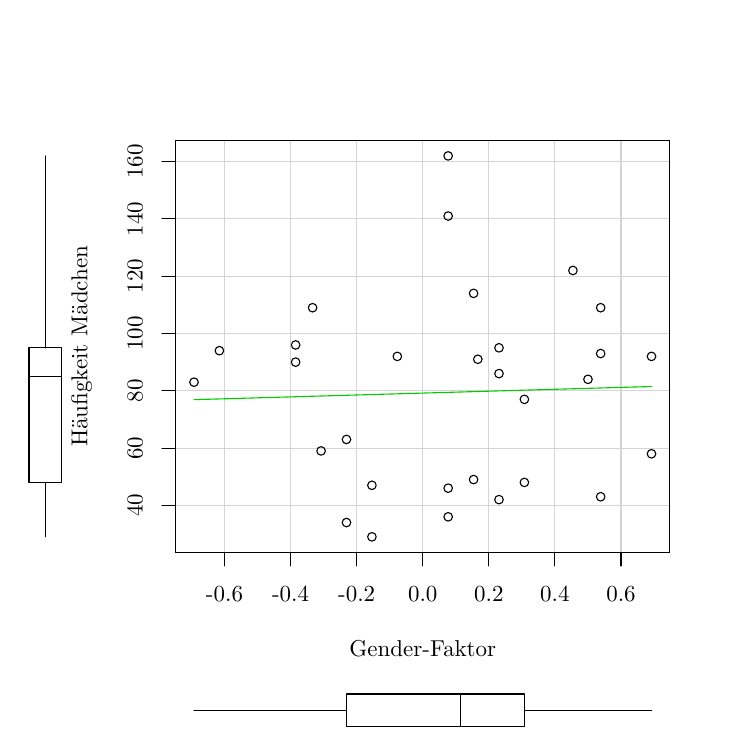
\begin{tikzpicture}[x=1pt,y=1pt]
\definecolor[named]{fillColor}{rgb}{1.00,1.00,1.00}
\path[use as bounding box,fill=fillColor,fill opacity=0.00] (0,0) rectangle (252.94,252.94);
\begin{scope}
\path[clip] (  0.00, 63.44) rectangle ( 12.65,212.11);
\definecolor[named]{drawColor}{rgb}{0.00,0.00,0.00}

\path[draw=drawColor,line width= 0.4pt,line join=round,line cap=round] (  0.47, 88.61) --
	( 12.18, 88.61) --
	( 12.18,137.26) --
	(  0.47,137.26) --
	(  0.47, 88.61);

\path[draw=drawColor,line width= 0.4pt,line join=round,line cap=round] (  0.47,126.91) --
	( 12.18,126.91);

\path[draw=drawColor,line width= 0.4pt,line join=round,line cap=round] (  6.32, 68.95) --
	(  6.32, 88.61);

\path[draw=drawColor,line width= 0.4pt,line join=round,line cap=round] (  6.32,137.26) --
	(  6.32,206.60);
\end{scope}
\begin{scope}
\path[clip] ( 53.48,  0.00) rectangle (232.03, 12.65);
\definecolor[named]{drawColor}{rgb}{0.00,0.00,0.00}

\path[draw=drawColor,line width= 0.4pt,line join=round,line cap=round] (115.20,  0.47) --
	(115.20, 12.18) --
	(179.49, 12.18) --
	(179.49,  0.47) --
	(115.20,  0.47);

\path[draw=drawColor,line width= 0.4pt,line join=round,line cap=round] (156.53,  0.47) --
	(156.53, 12.18);

\path[draw=drawColor,line width= 0.4pt,line join=round,line cap=round] ( 60.10,  6.32) --
	(115.20,  6.32);

\path[draw=drawColor,line width= 0.4pt,line join=round,line cap=round] (179.49,  6.32) --
	(225.42,  6.32);
\end{scope}
\begin{scope}
\path[clip] (  0.00,  0.00) rectangle (252.94,252.94);
\definecolor[named]{drawColor}{rgb}{0.00,0.00,0.00}

\path[draw=drawColor,line width= 0.4pt,line join=round,line cap=round] ( 71.12, 63.44) -- (214.39, 63.44);

\path[draw=drawColor,line width= 0.4pt,line join=round,line cap=round] ( 71.12, 63.44) -- ( 71.12, 58.46);

\path[draw=drawColor,line width= 0.4pt,line join=round,line cap=round] ( 95.00, 63.44) -- ( 95.00, 58.46);

\path[draw=drawColor,line width= 0.4pt,line join=round,line cap=round] (118.88, 63.44) -- (118.88, 58.46);

\path[draw=drawColor,line width= 0.4pt,line join=round,line cap=round] (142.76, 63.44) -- (142.76, 58.46);

\path[draw=drawColor,line width= 0.4pt,line join=round,line cap=round] (166.64, 63.44) -- (166.64, 58.46);

\path[draw=drawColor,line width= 0.4pt,line join=round,line cap=round] (190.52, 63.44) -- (190.52, 58.46);

\path[draw=drawColor,line width= 0.4pt,line join=round,line cap=round] (214.39, 63.44) -- (214.39, 58.46);

\node[text=drawColor,anchor=base,inner sep=0pt, outer sep=0pt, scale=  0.83] at ( 71.12, 45.52) {-0.6};

\node[text=drawColor,anchor=base,inner sep=0pt, outer sep=0pt, scale=  0.83] at ( 95.00, 45.52) {-0.4};

\node[text=drawColor,anchor=base,inner sep=0pt, outer sep=0pt, scale=  0.83] at (118.88, 45.52) {-0.2};

\node[text=drawColor,anchor=base,inner sep=0pt, outer sep=0pt, scale=  0.83] at (142.76, 45.52) {0.0};

\node[text=drawColor,anchor=base,inner sep=0pt, outer sep=0pt, scale=  0.83] at (166.64, 45.52) {0.2};

\node[text=drawColor,anchor=base,inner sep=0pt, outer sep=0pt, scale=  0.83] at (190.52, 45.52) {0.4};

\node[text=drawColor,anchor=base,inner sep=0pt, outer sep=0pt, scale=  0.83] at (214.39, 45.52) {0.6};

\path[draw=drawColor,line width= 0.4pt,line join=round,line cap=round] ( 53.48, 80.33) -- ( 53.48,204.53);

\path[draw=drawColor,line width= 0.4pt,line join=round,line cap=round] ( 53.48, 80.33) -- ( 48.50, 80.33);

\path[draw=drawColor,line width= 0.4pt,line join=round,line cap=round] ( 53.48,101.03) -- ( 48.50,101.03);

\path[draw=drawColor,line width= 0.4pt,line join=round,line cap=round] ( 53.48,121.73) -- ( 48.50,121.73);

\path[draw=drawColor,line width= 0.4pt,line join=round,line cap=round] ( 53.48,142.43) -- ( 48.50,142.43);

\path[draw=drawColor,line width= 0.4pt,line join=round,line cap=round] ( 53.48,163.13) -- ( 48.50,163.13);

\path[draw=drawColor,line width= 0.4pt,line join=round,line cap=round] ( 53.48,183.83) -- ( 48.50,183.83);

\path[draw=drawColor,line width= 0.4pt,line join=round,line cap=round] ( 53.48,204.53) -- ( 48.50,204.53);

\node[text=drawColor,rotate= 90.00,anchor=base,inner sep=0pt, outer sep=0pt, scale=  0.83] at ( 41.53, 80.33) {40};

\node[text=drawColor,rotate= 90.00,anchor=base,inner sep=0pt, outer sep=0pt, scale=  0.83] at ( 41.53,101.03) {60};

\node[text=drawColor,rotate= 90.00,anchor=base,inner sep=0pt, outer sep=0pt, scale=  0.83] at ( 41.53,121.73) {80};

\node[text=drawColor,rotate= 90.00,anchor=base,inner sep=0pt, outer sep=0pt, scale=  0.83] at ( 41.53,142.43) {100};

\node[text=drawColor,rotate= 90.00,anchor=base,inner sep=0pt, outer sep=0pt, scale=  0.83] at ( 41.53,163.13) {120};

\node[text=drawColor,rotate= 90.00,anchor=base,inner sep=0pt, outer sep=0pt, scale=  0.83] at ( 41.53,183.83) {140};

\node[text=drawColor,rotate= 90.00,anchor=base,inner sep=0pt, outer sep=0pt, scale=  0.83] at ( 41.53,204.53) {160};

\path[draw=drawColor,line width= 0.4pt,line join=round,line cap=round] ( 53.48, 63.44) --
	(232.03, 63.44) --
	(232.03,212.11) --
	( 53.48,212.11) --
	( 53.48, 63.44);
\end{scope}
\begin{scope}
\path[clip] ( 12.65, 12.65) rectangle (252.94,252.94);
\definecolor[named]{drawColor}{rgb}{0.00,0.00,0.00}

\node[text=drawColor,anchor=base,inner sep=0pt, outer sep=0pt, scale=  0.83] at (142.76, 25.60) {Gender-Faktor};

\node[text=drawColor,rotate= 90.00,anchor=base,inner sep=0pt, outer sep=0pt, scale=  0.83] at ( 21.61,137.78) {Häufigkeit Mädchen};
\end{scope}
\begin{scope}
\path[clip] ( 53.48, 63.44) rectangle (232.03,212.11);
\definecolor[named]{drawColor}{rgb}{0.83,0.83,0.83}

\path[draw=drawColor,line width= 0.4pt,line join=round,line cap=round] ( 71.12, 63.44) -- ( 71.12,212.11);

\path[draw=drawColor,line width= 0.4pt,line join=round,line cap=round] ( 95.00, 63.44) -- ( 95.00,212.11);

\path[draw=drawColor,line width= 0.4pt,line join=round,line cap=round] (118.88, 63.44) -- (118.88,212.11);

\path[draw=drawColor,line width= 0.4pt,line join=round,line cap=round] (142.76, 63.44) -- (142.76,212.11);

\path[draw=drawColor,line width= 0.4pt,line join=round,line cap=round] (166.64, 63.44) -- (166.64,212.11);

\path[draw=drawColor,line width= 0.4pt,line join=round,line cap=round] (190.52, 63.44) -- (190.52,212.11);

\path[draw=drawColor,line width= 0.4pt,line join=round,line cap=round] (214.39, 63.44) -- (214.39,212.11);

\path[draw=drawColor,line width= 0.4pt,line join=round,line cap=round] ( 53.48, 80.33) -- (232.03, 80.33);

\path[draw=drawColor,line width= 0.4pt,line join=round,line cap=round] ( 53.48,101.03) -- (232.03,101.03);

\path[draw=drawColor,line width= 0.4pt,line join=round,line cap=round] ( 53.48,121.73) -- (232.03,121.73);

\path[draw=drawColor,line width= 0.4pt,line join=round,line cap=round] ( 53.48,142.43) -- (232.03,142.43);

\path[draw=drawColor,line width= 0.4pt,line join=round,line cap=round] ( 53.48,163.13) -- (232.03,163.13);

\path[draw=drawColor,line width= 0.4pt,line join=round,line cap=round] ( 53.48,183.83) -- (232.03,183.83);

\path[draw=drawColor,line width= 0.4pt,line join=round,line cap=round] ( 53.48,204.53) -- (232.03,204.53);
\end{scope}
\begin{scope}
\path[clip] (  0.00,  0.00) rectangle (252.94,252.94);
\definecolor[named]{drawColor}{rgb}{0.00,0.00,0.00}

\path[draw=drawColor,line width= 0.4pt,line join=round,line cap=round] ( 53.48, 63.44) --
	(232.03, 63.44) --
	(232.03,212.11) --
	( 53.48,212.11) --
	( 53.48, 63.44);
\end{scope}
\begin{scope}
\path[clip] ( 53.48, 63.44) rectangle (232.03,212.11);
\definecolor[named]{drawColor}{rgb}{0.00,0.00,0.00}

\path[draw=drawColor,line width= 0.4pt,line join=round,line cap=round] (151.94, 86.54) circle (  1.55);

\path[draw=drawColor,line width= 0.4pt,line join=round,line cap=round] (124.39, 68.95) circle (  1.55);

\path[draw=drawColor,line width= 0.4pt,line join=round,line cap=round] (124.39, 87.58) circle (  1.55);

\path[draw=drawColor,line width= 0.4pt,line join=round,line cap=round] (161.13,156.92) circle (  1.55);

\path[draw=drawColor,line width= 0.4pt,line join=round,line cap=round] (161.13, 89.65) circle (  1.55);

\path[draw=drawColor,line width= 0.4pt,line join=round,line cap=round] (179.49, 88.61) circle (  1.55);

\path[draw=drawColor,line width= 0.4pt,line join=round,line cap=round] (202.46,125.87) circle (  1.55);

\path[draw=drawColor,line width= 0.4pt,line join=round,line cap=round] (102.96,151.75) circle (  1.55);

\path[draw=drawColor,line width= 0.4pt,line join=round,line cap=round] (151.94,206.60) circle (  1.55);

\path[draw=drawColor,line width= 0.4pt,line join=round,line cap=round] ( 69.28,136.22) circle (  1.55);

\path[draw=drawColor,line width= 0.4pt,line join=round,line cap=round] (151.94,184.87) circle (  1.55);

\path[draw=drawColor,line width= 0.4pt,line join=round,line cap=round] (106.02,100.00) circle (  1.55);

\path[draw=drawColor,line width= 0.4pt,line join=round,line cap=round] (179.49,118.63) circle (  1.55);

\path[draw=drawColor,line width= 0.4pt,line join=round,line cap=round] (207.05,151.75) circle (  1.55);

\path[draw=drawColor,line width= 0.4pt,line join=round,line cap=round] (162.66,133.12) circle (  1.55);

\path[draw=drawColor,line width= 0.4pt,line join=round,line cap=round] (115.20, 74.12) circle (  1.55);

\path[draw=drawColor,line width= 0.4pt,line join=round,line cap=round] (151.94, 76.19) circle (  1.55);

\path[draw=drawColor,line width= 0.4pt,line join=round,line cap=round] (133.57,134.15) circle (  1.55);

\path[draw=drawColor,line width= 0.4pt,line join=round,line cap=round] (170.31, 82.40) circle (  1.55);

\path[draw=drawColor,line width= 0.4pt,line join=round,line cap=round] ( 96.83,138.29) circle (  1.55);

\path[draw=drawColor,line width= 0.4pt,line join=round,line cap=round] (225.42,134.15) circle (  1.55);

\path[draw=drawColor,line width= 0.4pt,line join=round,line cap=round] ( 96.83,132.08) circle (  1.55);

\path[draw=drawColor,line width= 0.4pt,line join=round,line cap=round] (207.05, 83.44) circle (  1.55);

\path[draw=drawColor,line width= 0.4pt,line join=round,line cap=round] ( 60.10,124.84) circle (  1.55);

\path[draw=drawColor,line width= 0.4pt,line join=round,line cap=round] (170.31,137.26) circle (  1.55);

\path[draw=drawColor,line width= 0.4pt,line join=round,line cap=round] (207.05,135.19) circle (  1.55);

\path[draw=drawColor,line width= 0.4pt,line join=round,line cap=round] (170.31,127.94) circle (  1.55);

\path[draw=drawColor,line width= 0.4pt,line join=round,line cap=round] (225.42, 98.96) circle (  1.55);

\path[draw=drawColor,line width= 0.4pt,line join=round,line cap=round] (197.03,165.20) circle (  1.55);

\path[draw=drawColor,line width= 0.4pt,line join=round,line cap=round] (115.20,104.14) circle (  1.55);
\definecolor[named]{drawColor}{rgb}{0.00,0.80,0.00}

\path[draw=drawColor,line width= 0.4pt,line join=round,line cap=round] ( 60.10,118.52) --
	(225.42,123.27);
\end{scope}
\end{tikzpicture}
